\documentclass[tikz,border=10pt]{standalone}
\usepackage{tikz}
\usetikzlibrary{positioning,arrows.meta,shapes.geometric,calc}

\begin{document}
	
	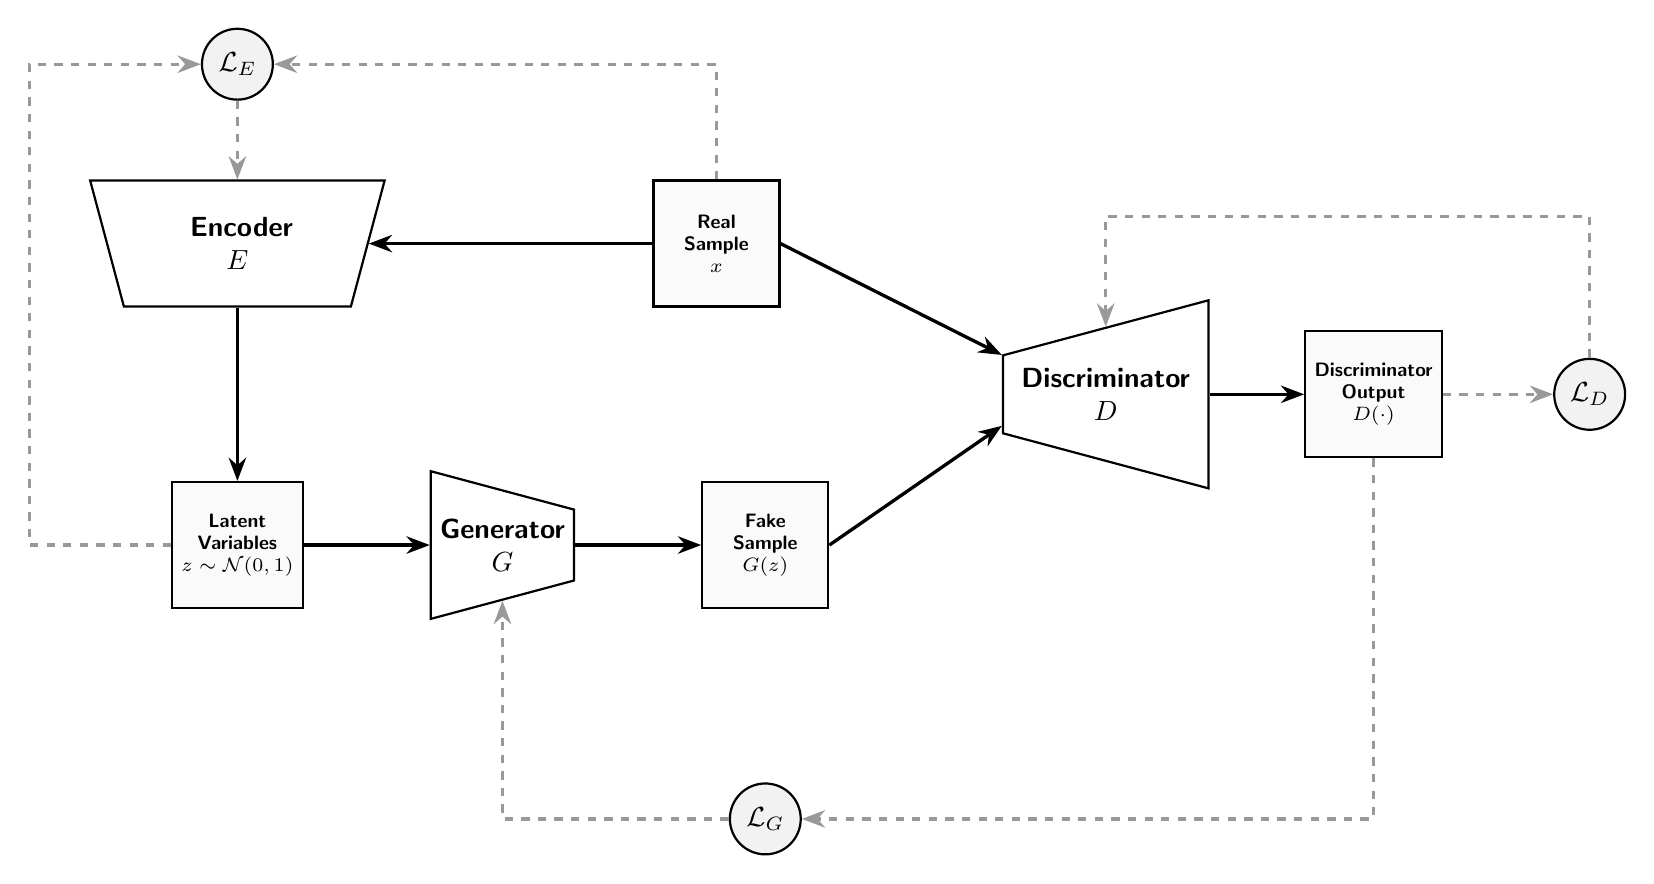
\begin{tikzpicture}[
		>=Stealth,
		node distance=1.2cm and 1.6cm,
		thick,
		generator_wedge/.style={
			trapezium, trapezium left angle=75, trapezium right angle=75, shape border rotate=270,
			draw=black, fill=white, minimum width=1.6cm, minimum height=1.8cm, font=\sffamily\bfseries,
			align=center
		},
		discriminator_wedge/.style={
			trapezium, trapezium left angle=75, trapezium right angle=75, shape border rotate=90,
			draw=black, fill=white, minimum width=2.4cm, minimum height=1.8cm, font=\sffamily\bfseries,
			align=center
		},
		encoder_wedge/.style={
			trapezium, trapezium left angle=75, trapezium right angle=75, shape border rotate=180,
			draw=black, fill=white, minimum width=1.4cm, text width=1.2cm, minimum height=1.6cm, font=\sffamily\bfseries,
			align=center, inner sep=0pt
		},
		image/.style={rectangle, draw=black, fill=black!2, minimum size=1.6cm, font=\scriptsize\sffamily\bfseries, align=center},
		loss_node/.style={circle, draw=black, fill=black!5, minimum size=0.9cm, font=\sffamily\bfseries, align=center}
		]
		
		% --- CORE VERTICAL AXIS (Latent Variables & Encoder) ---
		% 1. Central Latent Variable Repository
		\node[image] (z) {Latent\\Variables\\$z \sim \mathcal{N}(0,1)$};
		
		% 2. Encoder Wedge (Bound tightly by explicit text width constraints)
		\node[encoder_wedge, above=2.2cm of z] (E) {Encoder\\$E$};
		
		
		% --- GENERATOR TRACK ---
		% 3. Generator
		\node[generator_wedge, right=of z] (G) {Generator\\$G$};
		
		% 4. Generated Fake Data
		\node[image, right=of G] (x_fake) {Fake\\Sample\\$G(z)$};
		
		
		% --- REAL DATA TRACK ---
		\node[image, right=3.6cm of E] (x_real) {Real\\Sample\\$x$};
		
		
		% --- DISCRIMINATOR TRACK ---
		\path (x_real.east) -- (x_fake.east) coordinate[midway] (mid_data);
		\node[discriminator_wedge, right=2.5cm of mid_data] (D) {Discriminator\\$D$};
		
		
		% --- OUTPUT AND LOSS NODES POSITIONED FOR ZERO OVERLAP ---
		\node[image, right=1.2cm of D] (D_out) {Discriminator\\Output\\$D(\cdot)$};
		
		% Loss Nodes
		\node[loss_node, above=1.0cm of E] (L_E) {$\mathcal{L}_E$};
		\node[loss_node, right=1.4cm of D_out] (L_D) {$\mathcal{L}_D$};
		\node[loss_node, below=2.2cm of x_fake] (L_G) {$\mathcal{L}_G$};
		
		
		% --- FORWARD CONNECTIONS AND FLOW (Solid Black Lines) ---
		% 1. Reconstruction Loop (Real Sample enters Encoder, Encoder points straight down to Latent)
		\draw[->, line width=1.2pt] (x_real.west) -- (E.east);
		\draw[->, line width=1.2pt] (E.south) -- (z.north);
		
		% 2. Generator Path (Left to Right)
		\draw[->, line width=1.2pt] (z.east) -- (G.west);
		\draw[->, line width=1.2pt] (G.east) -- (x_fake.west);
		
		% 3. Discriminator Symmetric Inflow
		\draw[->, line width=1.2pt] (x_real.east) -- ([yshift=0.5cm]D.west);
		\draw[->, line width=1.2pt] (x_fake.east) -- ([yshift=-0.4cm]D.west);
		
		% 4. Discriminator to Prediction Block (Solid Forward Path)
		\draw[->, line width=1.2pt] (D.east) -- (D_out.west);
		
		
		% --- BACKPROPAGATION TRACKS  ---
		\draw[->, dashed, line width=1.2pt, draw=black!40] (D_out.east) -- (L_D.west);
		
		\draw[->, dashed, line width=1.2pt, draw=black!40] (L_D.north) |- ([yshift=1.4cm]D.north) -- (D.north);
		
		\draw[->, dashed, line width=1.2pt, draw=black!40] (D_out.south) |- (L_G.east);
		
		\draw[->, dashed, line width=1.2pt, draw=black!40] (L_G.west) -| (G.south);
		
		\draw[->, dashed, line width=1.2pt, draw=black!40] (L_E.south) -- (E.north);
		
		\draw[->, dashed, line width=1.2pt, draw=black!40] (z.west) -- ++(-1.8,0) |- (L_E.west);
		
		\draw[->, dashed, line width=1.2pt, draw=black!40] (x_real.north) -- ++(0,1.0) |- (L_E.east);
		
	\end{tikzpicture}
\end{document}
